% ============================================================
% Lecture deck — Module 8 / Notebook 30
% AI-Assisted Software Development. HSBI house style. TikZ visuals.
% The notebook is the single source of truth.
% ============================================================
\documentclass[aspectratio=169,11pt]{beamer}

\usepackage[utf8]{inputenc}
\usepackage[T1]{fontenc}
\usepackage{lmodern}
\usepackage[english]{babel}
\usepackage{graphicx}
\usepackage{booktabs}
\usepackage{amsmath,amssymb}
\usepackage{xcolor}
\usepackage{tikz}
\usetikzlibrary{positioning,arrows.meta,shapes.geometric,calc,fit,backgrounds}

\usetheme{Madrid}
\usecolortheme{default}
\setbeamertemplate{navigation symbols}{}
\setbeamertemplate{footline}[frame number]
\setbeamertemplate{blocks}[rounded][shadow=false]
\setbeamertemplate{headline}{%
  \leavevmode%
  \hbox{%
    \begin{beamercolorbox}[wd=\paperwidth,ht=2.5ex,dp=1.125ex]{section in head/foot}%
      \insertsectionnavigationhorizontal{\paperwidth}{}{\hskip0pt plus1filll}%
    \end{beamercolorbox}%
  }%
}
\AtBeginSection[]{%
  \begin{frame}{Outline}
    \tableofcontents[currentsection,sectionstyle=show/shaded,subsectionstyle=show/show/hide]
  \end{frame}
}

\definecolor{hsbiblue}{RGB}{45,57,120}
\definecolor{hsbimid}{RGB}{76,114,176}
\definecolor{hsbilight}{RGB}{225,231,247}
\definecolor{cgreen}{RGB}{85,164,103}
\definecolor{corange}{RGB}{221,132,82}
\definecolor{cred}{RGB}{196,78,82}
\definecolor{cpurple}{RGB}{129,114,178}
\tikzset{
  box/.style={rounded corners=3pt, draw=hsbiblue, line width=1pt, fill=hsbilight, align=center, inner sep=5pt, font=\footnotesize},
  modebox/.style={rounded corners=3pt, draw=hsbiblue, line width=1.1pt, fill=hsbilight, align=center, text width=2.7cm, minimum height=1.5cm, font=\scriptsize},
  cyc/.style={rounded corners=3pt, draw=hsbiblue, line width=1.1pt, fill=hsbilight, align=center, text width=2.2cm, minimum height=0.9cm, font=\scriptsize},
  arr/.style={-{Stealth[length=2.6mm]}, line width=1pt, draw=hsbiblue},
}

\title{AI-Assisted Software Development}
\subtitle{Module 8 --- Business AI in Practice $\cdot$ Notebook 30}
\author{Prof.\ Dr.\ Christoph Weisser}
\institute{HSBI}
\date{Summer Semester 2026}

\begin{document}

\begin{frame}\titlepage\end{frame}

\begin{frame}{Contents}
  \tableofcontents[hideallsubsections]
\end{frame}

% ============================================================
\section{IDEs}
% ============================================================
\begin{frame}{The modern IDE landscape (2026)}
  \small
  \begin{center}
  \begin{tabular}{lp{4.4cm}p{3.6cm}}
    \toprule
    \textbf{Tool} & \textbf{AI assistance} & \textbf{Best for} \\
    \midrule
    VS Code $+$ Copilot & inline completion $+$ chat & broad default; Jupyter support \\
    Cursor              & chat-first; multi-file refactors & agentic edits, big rewrites \\
    PyCharm $+$ JetBrains AI & completion $+$ assistant panel & large, refactor-heavy projects \\
    \bottomrule
  \end{tabular}
  \end{center}
  \begin{exampleblock}{Recommendation for beginners}
    \textbf{VS Code $+$ Copilot} or \textbf{Cursor} --- the most forgiving combinations to learn the workflow on.
  \end{exampleblock}
\end{frame}

\begin{frame}{Three ways the assistant helps --- rising autonomy}
  \begin{center}
  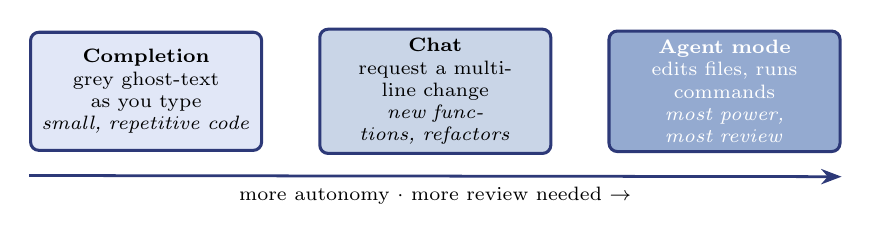
\begin{tikzpicture}
    \node[modebox, fill=hsbilight]  (c) {\textbf{Completion}\\ grey ghost-text as you type\\ \emph{small, repetitive code}};
    \node[modebox, fill=hsbimid!30, right=0.7cm of c] (h) {\textbf{Chat}\\ request a multi-line change\\ \emph{new functions, refactors}};
    \node[modebox, fill=hsbimid!60, right=0.7cm of h, text=white] (a) {\textbf{Agent mode}\\ edits files, runs commands\\ \emph{most power, most review}};
    \draw[arr] ($(c.south west)+(0,-0.3)$) -- ($(a.south east)+(0,-0.3)$)
      node[midway,below,font=\scriptsize]{more autonomy $\cdot$ more review needed $\to$};
  \end{tikzpicture}
  \end{center}
  {\footnotesize The more the assistant does on its own, the more your review discipline matters (Module 9 builds on Agent mode).}
\end{frame}

% ============================================================
\section{Git}
% ============================================================
\begin{frame}{Git --- nine commands cover 90\,\% of daily work}
  \small
  \begin{center}
  \begin{tabular}{ll}
    \toprule
    \textbf{Command} & \textbf{What it does} \\
    \midrule
    \texttt{status} / \texttt{diff}          & see what changed \\
    \texttt{add} / \texttt{commit}           & stage and snapshot \\
    \texttt{pull} / \texttt{push}            & sync with the remote \\
    \texttt{checkout -b} / \texttt{checkout} & make / switch a branch \\
    \texttt{merge}                            & combine a branch back in \\
    \bottomrule
  \end{tabular}
  \end{center}
  \begin{alertblock}{Common beginner mistake}
    \emph{Force-pushing} over the main branch destroys history others built on. Force-push only your \emph{own} feature branches.
  \end{alertblock}
\end{frame}

\begin{frame}{Branches and pull requests --- the unit of professional work}
  \begin{center}
  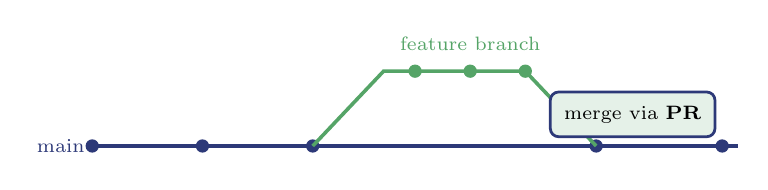
\begin{tikzpicture}[scale=1]
    % main line
    \draw[line width=1.3pt, hsbiblue] (0,0) -- (8.2,0);
    \foreach \x in {0,1.4,2.8,6.4,8}{\fill[hsbiblue] (\x,0) circle(2.4pt);}
    \node[font=\scriptsize, hsbiblue] at (-0.4,0) {main};
    % feature branch
    \draw[line width=1.3pt, cgreen] (2.8,0) -- (3.7,0.95) -- (5.5,0.95) -- (6.4,0);
    \foreach \x in {4.1,4.8,5.5}{\fill[cgreen] (\x,0.95) circle(2.4pt);}
    \node[font=\scriptsize, cgreen] at (4.8,1.3) {feature branch};
    \node[box, fill=cgreen!15, font=\scriptsize, above right=0.1cm and -0.6cm of {(6.4,0)}] {merge via \textbf{PR}};
  \end{tikzpicture}
  \end{center}
  \begin{block}{A good PR}
    short title $\cdot$ a 2-paragraph \emph{what / why / tested} $\cdot$ \textbf{small scope} (30 lines reviewed in 5 min) $\cdot$ tests or a screenshot.
  \end{block}
  {\footnotesize AI-generated PRs are no exception --- arguably \emph{more} important to keep small.}
\end{frame}

% ============================================================
\section{Prompting}
% ============================================================
\begin{frame}{Five prompt patterns for code}
  \begin{enumerate}
    \item \textbf{Give it what it can't see} --- the surrounding code, the schema, the error.
    \item \textbf{Ask for one thing}, explicitly --- one change per turn, then iterate.
    \item \textbf{Be specific about constraints} --- version, libraries, style, performance, error semantics.
    \item \textbf{Ask for tests} --- ``add a pytest for the empty-input case.''
    \item \textbf{Ask for alternatives when designing} --- ``three storage options with trade-offs.''
  \end{enumerate}
\end{frame}

\begin{frame}{Prompting is a loop, not a one-shot}
  \begin{center}
  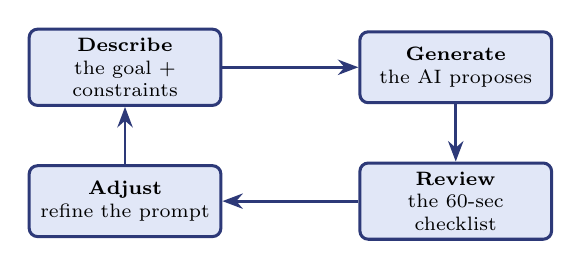
\begin{tikzpicture}
    \node[cyc] (d) at (0,1.7) {\textbf{Describe}\\ the goal + constraints};
    \node[cyc] (g) at (4.2,1.7) {\textbf{Generate}\\ the AI proposes};
    \node[cyc] (r) at (4.2,0) {\textbf{Review}\\ the 60-sec checklist};
    \node[cyc] (a) at (0,0) {\textbf{Adjust}\\ refine the prompt};
    \draw[arr] (d) -- (g);
    \draw[arr] (g) -- (r);
    \draw[arr] (r) -- (a);
    \draw[arr] (a) -- (d);
  \end{tikzpicture}
  \end{center}
  {\footnotesize Each turn is small and reviewable. You stay the author --- the assistant drafts; you decide.}
\end{frame}

% ============================================================
\section{Review}
% ============================================================
\begin{frame}{Four failure modes of AI-generated code}
  \begin{center}
  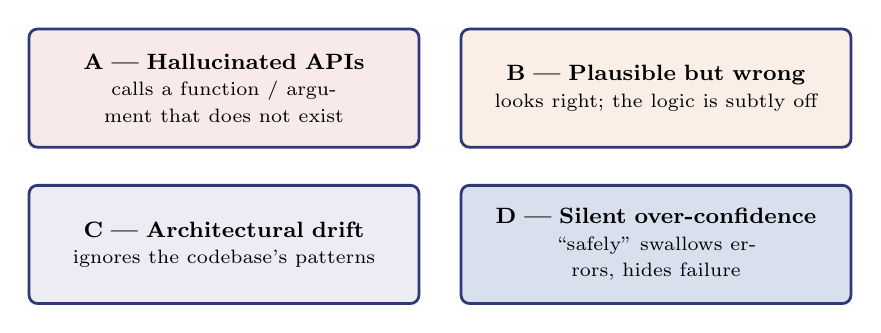
\begin{tikzpicture}
    \node[box, fill=cred!12,    text width=4.6cm, minimum height=1.5cm] (A) {\textbf{A --- Hallucinated APIs}\\ \scriptsize calls a function / argument that does not exist};
    \node[box, fill=corange!14, text width=4.6cm, minimum height=1.5cm, right=0.5cm of A] (B) {\textbf{B --- Plausible but wrong}\\ \scriptsize looks right; the logic is subtly off};
    \node[box, fill=cpurple!14, text width=4.6cm, minimum height=1.5cm, below=0.45cm of A] (C) {\textbf{C --- Architectural drift}\\ \scriptsize ignores the codebase's patterns};
    \node[box, fill=hsbimid!22, text width=4.6cm, minimum height=1.5cm, below=0.45cm of B] (D) {\textbf{D --- Silent over-confidence}\\ \scriptsize ``safely'' swallows errors, hides failure};
  \end{tikzpicture}
  \end{center}
\end{frame}

\begin{frame}{The 60-second review checklist}
  \begin{block}{Run this on every AI-generated change before you accept or merge}
    \begin{enumerate}
      \item \textbf{Does it run?} Even just the import line.
      \item \textbf{Are there tests?} If not, ask for them.
      \item \textbf{Does it use our libraries / patterns?} Grep for one similar function.
      \item \textbf{Does it swallow errors?} Search the diff for \texttt{except Exception}, \texttt{or \{\}}, \texttt{pass}.
      \item \textbf{Does it do exactly what was asked} --- no more, no less?
    \end{enumerate}
  \end{block}
  {\footnotesize 60 seconds; catches $\approx$80\,\% of failures. The rest is what real testing and code review are for.}
\end{frame}

% ============================================================
\section{When not}
% ============================================================
\begin{frame}{When \emph{not} to use the AI assistant}
  \begin{exampleblock}{Mental model}
    AI assistants are most valuable when you \emph{could} write the code yourself but would rather not. They are least valuable when you don't yet understand the problem.
  \end{exampleblock}
  \begin{itemize}
    \item Skip it when the task is to \emph{learn} the concept --- write the first version yourself.
    \item Skip it for security- / correctness-critical logic you can't fully review.
    \item \textbf{Companion notebook:} hands-on Git, PR, and review exercises are in \textbf{Notebook 30} --- recommended \emph{early} so the workflow pays off everywhere.
  \end{itemize}
\end{frame}

\end{document}
